\section{Data}
%% Version 1 (Score 100)
We evaluated the performance of our model on a custom dataset that imitated Zoom sessions under various channel bandwidths (changed with the NetLimitter application). It included network channel data pickup from 720 controlled Zoom sessions, where the features in \cref{tab:zoom-features} were collected and averaged over one second to decrease the noise.

% To test the performance of our models, we created a labeled dataset of Zoom calls, where we used the Netlimitter traffic control software to limit the bandwidth of the channel, to simulate various network conditions. The dataset contains 720 samples, where each sample is an average over the measurements over 1 sec taken while modifying channels' bandwidth.
% and for each of the samples different parameters were extracted from the encrypted traffic, e.g., bandwidth, resolution, FPS, latency etc. 
% We train ML algorithms to predict QoE metrics from encrypted Zoom video conferencing traffic. To accomplish that, we have created a dataset of labeled samples. In order to assess the Zoom video quality degradation and build a suitable dataset to predict it, we studied the behavior of the Zoom video session under changing network channel conditions. Analyzing the Zoom behavior pattern, we realized that the focus should be on the transition periods, where the spatial as well as the temporal resolutions are interchangeably affected. Each sample in our dataset is averaged over a 1 sec interval taken while modifying the channel bandwidth by the Netlimiter traffic control software. For each data sample we captured the features and the labels. Our dataset includes 720 samples and can be downloaded from https://github.com/yogevdrori/Encrypted-Zoom-traffic-dataset.git.



\subsection{Features}
Zoom provides several metrics available for the end user through its' Software Developer Kit (SDK), which may be automatically extracted from the session stream in real time. For our dataset we captured all them, as we wanted to explore their predictive ability of the QoE. All the features in our dataset are listed in \cref{tab:zoom-features}.

\begin{table*}
    \caption{Features extracted from the encrypted Zoom traffic for the dataset}
    \centering
        \begin{tabular}{l|l}
            Feature & Description \\        
            \hline
            Bandwidth & \makecell[l]{The number of bits per second allowed to be\\transmitted on the channel}\\
            Resolution & \makecell[l]{The number of pixels in the width and the\\length of the presented image}\\
            FPS & The number of frames per second in the playback\\
            Latency & Initial time after which the video starts\\
            Jitter & \makecell[l]{Statistical variance of the Real-time Transport Protocol (RTP)\cite{schulzrinne2003rfc3550}\\data packet in time interval}\\
            PPS & Number of transmitted packets in each second\\
            Destination port & \makecell[l]{The $2^{nd}$ layer port on the remote host where\\ the transmitted data is directed to}\\
            Source port & \makecell[l]{The $2^{nd}$ layer port on the local host through which\\the data is transmitted}\\
            \makecell[l]{Average time\\between packets} & \makecell[l]{The time difference between the reception of two\\consecutive packets}\\
            Packet length & Number of bytes in each transmitted packet\\
        \end{tabular} 
    \label{tab:zoom-features}
\end{table*}

\subsection{The QoE Metric}
In our experiments we used the Naturallness Image Quality Evaluator (NIQE) metric proposed \cite{mittal2012making}.  
% Just by looking at an image, or a video, we can asses its' quality fairly quickly. However finding an objective criterion for quality assessment is a challenging task for an automated system. Many lines of work tried to propose their criteria for a numeric quality measure, but all divide into two categories, viz. Full Reference (FR) and No Reference (NR) QoE metrics. The difference between the two may be summarized in the fact that while the former requires human assessment, the latter uses algorithmic approach to achieve the quality criterion. In this work we chose to concentrate on one metric from each category, i.e., the Video Multi-method Assessment Fusion (VMAF) \cite{li2016toward} as the FR QoE metric, whereas for the NR metric we chose the Naturalness Image Quality Evaluator (NIQE) \cite{mittal2012making}.

% \subsection{VMAF metric}
% This metric was developed by Netflix as an alternative to the Peak Signal-to-Noise Ratio (PSNR) metric which is defined via the Mean Squared Error (MSE) of the original image $I$ and the lossy image $L$ as is shown in \cref{eq:mse} and \cref{eq:psnr}.
 
% \begin{equation}
%     MSE[I, L] = \frac{1}{mn}\sum_{i=0}^{m-1}\sum_{j=0}^{n-1}[I(i, j) - L(i, j)]^2
%     \label{eq:mse}
% \end{equation}
% \begin{equation}
%     PSNR = 10 log_{10}(\frac{MAX_I^2}{MSE})
%     \label{eq:psnr}
% \end{equation}

% As the authors of \cite{li2016toward} maintain that PSNR does not provide a reliable criterion for the QoE assessment. They develop the VMAF as a Machine Learning (ML) based metric, which teaches a Support Vector Machine (SVM) model on three basic metrics, i.e., two for image quality, viz. Visual Information Fidelity (VIF) \cite{sheikh2006image} and the Detail Loss Metric (DLM) \cite{li2011image}, and one for temporal quality assessment, viz. Motion, which performs a simple average of absolute differences of pixel wise intensities between two consecutive frames. 

% VMAF uses as labels human assessment on video fragments corrupted with noise with the corresponding clean reference video fragment (i.e., without noise added). Human evaluators rate the corrupted video fragment on a scale of 1 to 5 (i.e., where 1 means "very annoying" while 5 is "not noticeable"). Than the scores for each video and from every evaluator are combined and normalized to form the Differential Mean Opinion Score (DMOS) which lays in the range of [0, 100], where the score of 100 given for the reference video.
% We extracted several FR video quality metrics from Zoom traffic. In order to assess the quality degradation caused by reduced bandwidths, we needed to compare a reference source video of original quality to the same video stream at the receiving end, that was impacted by the network conditions. We have access to the video that is recorded by the Zoom application. We observed that when establishing a 2-party conference call, Zoom reduces the quality of the recorded video at the source and at the destination at the same time. In order to obtain a good quality reference, we managed to force the Zoom application to produce and record a good quality video. This was accomplished by adding to the call a 3rd party without a bandwidth limitation. This way the sending Zoom application allows to record a good quality reference which is not impacted by the restricted bandwidth of the 2nd party to the call. The setup used to record the reference and the destination videos is depicted in \Cref{fig:vmaf-setup}. In order to perform a reasonably accurate comparison between the 2 recorded streams, they have to be synchronized. We used the audio recording to synchronize the streams by creating an abrupt loud instantaneous noise (similar to "cut" used in recording a movie "video take") and synchronized the videos at the sender and recipient ends using that noise.
% The results of the Full reference video QoE metrics measured using the setup depicted in \Cref{fig:vmaf-setup} are provided in \Cref{fig:qual-metrics}. The slight improvement of quality observed when the bandwidth is decreased can be explained by the slight decrease of the Qp parameter performed by Zoom during the bandwidth drop transition period (depicted in \Cref{fig:adapt-patt}). It is assumed that Zoom decreases the Qp to compensate for reduced quality during the bandwidth drop transition.

\subsection{NIQE Metric}
Due to the challenges of recording Zoom video sessions with FR and in order to make the dataset more accommodating to future expansions (which do not necessitate complicate setups and saving of a reference for each recorded video clip), we researched the No Reference (NR) QoE metric alternatives. A promising NR metric that has emerged is the Naturalness Image Quality Evaluator (NIQE) \cite{mittal2012making}, which measures the distance of the frame from naturalness, therefore, a smaller score indicates better perceptual quality. NIQE measures the distance between the Natural Scene Statistics (NSS)-based features calculated from an image to the features obtained from an image database used to train the model. The features are modeled as multidimensional Gaussian distributions. We calculated NIQE as a function of bandwidth, resolution and FPS. The corresponding graphs are depicted in \Cref{fig:niqe-fps-bw-res}. As can be seen in \Cref{fig:niqe-fps-bw-res} (b) and (c), the NIQE is consistent with available bandwidth and video frame resolution respectively, such that the larger the bandwidth or the resolution, the smaller the NIQE, thus indicating better quality.  We can observe a range of resolutions for which the NIQE value remains constant, indicating that the image naturalness metric at these resolutions is sufficiently good despite the change. An interesting observation is depicted in \Cref{fig:niqe-fps-bw-res} (a), indicating a change of NIQE with FPS, whereas the metric is measured per single frame and is therefore spatial by nature. The temporal resolution of the video frames has an impact on the spatial quality. This is due to the compression algorithm that utilizes quantized residuals which are determined by block prediction accuracy, which is in turn impacted by the magnitude of the Motion Vectors (MV) used for Inter-prediction. The larger the movement between consecutive frames, the larger the MV magnitude and the less accurate is the prediction, thus increasing the value of the temporary predicted block residuals and reducing the quality due to their quantization.

% This metric is based on the assumption that natural images (i.e., images which represent objects commonly observed in nature), and the features contained in them, may be expressed by features that follow the Multi-Variate Gaussian(MVG) \nomenclature{MVG}{Multi-Variate Gaussian} model. 

% This QoE technique expresses the image as a collection of quality-aware features, i.e., features that are derived from a simple, but highly regular Natural Scene Statistics (NSS) \nomenclature{NSS}{Natural Scene Statistics} model \cite{ruderman1993statistics} that are fitted to the MVG; an example for such a feature may be expresses as a local mean and contrast estimation with a MVG of some normalized (i.e., by removing the mean and dividing by a standard deviation of pixel values) image patch $I$, as shown in \cref{eq: niqe-feat-mu} and \cref{eq: niqe-feat-sigma}, where $\hat{I}(i,j) = \frac{I(i,j) - \mu(i,j)}{\sigma(i,j) + 1}$, and $w = \{ w_{l,k | k = -K,...,K, l = -L,...,L}\}$, which is a 2D circularly-symmetric Gaussian weighting function sampled out 3 standard deviations and rescaled to unit volume (i.e., $K=L=3$).

% \begin{equation}
%     \mu(i, j) = \sum\limits_{k=-K}^{K}\sum\limits_{l=-L}^{L}w_{k,l}\hat{I}(i+k, j+l)
%     \label{eq: niqe-feat-mu}
% \end{equation}

% \begin{equation}
%     \sigma(i, j) = \sqrt{\sum\limits_{k=-K}^{K}\sum\limits_{l=-L}^{L}w_{k,l}\left[\hat{I}(i+k, j+l) - \mu(i,j)\right]^2}
%     \label{eq: niqe-feat-sigma}
% \end{equation}

% Finlay, NIQE is expressed by the mean distance of the collection of the NSS features extracted from image patches to the NSS features extracted from the corpus of natural images

% \subsection{Labels}
% Zoom provides several metrics available for the end user through its' Software Developer Kit (SDK), which may be automatically extracted from the session stream in real time, and latter used as labels for the supervised model training. 
% The User Interface (UI) of the Zoom application provides several QoE metrics. We used the Zoom Software Developers Kit (SDK) to extract these metrics programmatically and used them as labels. The Labels that we extracted from Zoom and used as QoE metrics are latency, Jitter, Resolution, and frames per second (fps). The predominant parameters used by the Zoom application when adapting to network channel conditions are Spatial and Temporal resolutions, whereas the spatial resolution is the frame image pixels density and the temporal resolution is the frame rate, measured in frames per second (fps). The Zoom SDK screen that indicates these labels is depicted in \Cref{fig:qoe-from-app}. The application captures the quality metrics at the sending and at the receiving end. We noticed that the resolution is also impacted by the size of the video window selected by the user – in the case of a smaller video window, the resolution is reduced and in the case of a larger window, it is increased.
% In addition to the quality metrics that are extracted directly from the Zoom application, we also used additional video QoE metrics. We built a setup to capture Full Reference (FR) metrics \Cref{fig:exp-setup},  such as VMAF ‎\cite{li2018vmaf} and also implemented No Reference (NR) metrics such as NIQE ‎\cite{mittal2012making}.
\subsection{Exploratory Data Analysis (EDA)}
\label{sec:eda}
First, we performed a simple Pearson correlation \cite{pearson1895vii} of the extracted features, which is listed in \cref{tab:corr_table}. This analysis highlighted the features which influence the target (i.e., the NIQE), the most. Pearson correlation is a measure of the influence which some feature $X$ has on its' counterpart $Y$, i.e., how precisely can we anticipate a change (positive or negative) in $Y$ by observing $X$, and is defined as 

\begin{equation}
    \rho_{X,Y} = \frac{Cov[X,Y]}{\sigma(X)\sigma(Y)}
\label{eq:pearson_cor}
\end{equation}
This measure is located in the range [-1, 1], where 1 points to a perfect positive correlation, i.e., increase in one feature brings increase in the other, while -1 signifies a total reverse correlation, accordingly, which may be seen in \Cref{tab:corr_table}. Features with correlation closer to $\pm{1}$ are the most interesting, as it indicates that this feature, or it reverse, has strong effect on the predicted variable. 
Among the strongest predictive values we see \emph{bandwidth} (-0.78), \emph{resolution} (-0.73), \emph{FPS} (-0.76), \emph{average time between packets} (0.77), and surprisingly, also \emph{packet length} (-0.86). 

As for the first three, its is quite intuitive that increase in their value will decrease the NIQE, as higher bandwidth leads directly to better resolution and fps, which in its' turn improves the perceived quality of the video. 

The \emph{average time between packets}, which has a strong positive correlation with NIQE, i.e., increase in this feature leads to worse QoE of the observer (as a high NIQE means worse QoE than a low one). This is also intuitively clear, as packages which arive at a lower rate may indicate a lower FPS.

The high negative correlation of the \emph{packet length} though is less intuitive, but yet has an explanation, viz. as we increase the bandwidth, video compressor has the ability to place more data in each packet, increasing the FPS, and by this increasing also the QoE of the viewer.

In addition, to reduce the dimensionality of our dataset even further, we performed the the Primary Component Analysis (PCA) \cite{pearson1901liii} algorithm, which may be seen as a method to project the data to a lower dimensional subspace, but one that still contain most of the information from the original space. The results of this procedure are presented in \cref{fig:pca}, and in the corresponding \cref{tab:pca_loadings}.
% on the features in our dataset to acquire a subspace where the features will be sorted by their importance \Cref{fig:pca}.
From this analysis we conclude that the by transforming the features with the corresponding loadings, we can use as few as 5 features instead of the 9 original and still retain 99\% of the information present in the data.


\begin{table*}[t]
    \caption{Pearson correlation of different features in the dataset. In bold script are the features with the largest positive or negative correlation with the explained feature, i.e., NIQE}
    \centering
    \scalebox{0.8}{
        \begin{tabular}{l|c|c|c|c|c|c|c|c|c|c|c}
             & BW & NIQE & Resolution & FPS & Latency & Jitter & PPS & Destination & Source & Average time & Packet\\
             & & & & & &  & & Port & Port & between packets & Length\\
             \hline
             \textbf{BW} & 1.0 & \textbf{-0.777} & 0.586 & 0.656 & -0.274 & -0.383 & 0.946 & -0.032 & 0.056 & -0.931 & 0.873\\
             NIQE & -0.777 & 1.0 & -0.728 & -0.758 & 0.391 & 0.486 & -0.666 & 0.067 & -0.088 & 0.770 & -0.860\\
             \textbf{Resolution} & 0.586 & \textbf{-0.728} & 1.0 & 0.765 & -0.417 & -0.458 & 0.493 & -0.111 & 0.132 & -0.593 & 0.719\\
             \textbf{FPS} & 0.656 & \textbf{-0.758} & 0.765 & 1.0 & -0.478 & -0.495 & 0.591 & -0.071 & 0.094 & -0.679 & 0.693\\
             Latency & -0.274 & 0.391 & -0.417 & -0.478  & 1.0 & -0.798 & -0.231 & 0.042 & -0.061 & 0.284 & -0.359\\
             Jitter & -0.383 & 0.486 & -0.458 & -0.495  & -0.798 & 1.0 & -0.328 & 0.018 & -0.040 & 0.377 & -0.467\\
             \textbf{PPS} & 0.946 & \textbf{-0.666} & 0.493 & 0.591  & -0.231 & -0.328 & 1.0 & 0.022 & 0.004 & -0.933 & 0.721\\
             Destination Port & -0.032 & 0.067 & -0.111 & -0.071  & 0.042 & 0.018 & 0.022 & 1.0 & -0.985 & 0.012 & -0.074\\
             Source Port & 0.056 & -0.088 & 0.132 & 0.094  & -0.061 & -0.040 & 0.004 & -0.985 & 1.0 & -0.044 & 0.106\\
             \makecell[l]{\textbf{Average time}\\\textbf{between packets}} & -0.931 & \textbf{0.770} & -0.593 & -0.679  & 0.284 & 0.377 & -0.933 & 0.012 & -0.044 & 1.0 & -0.783\\
             \textbf{Packet length} & 0.873 & \textbf{-0.860} & 0.719 & 0.693  & -0.359 & -0.467 & 0.721 & -0.074 & 0.106 & -0.783 & 1.0\\
        \end{tabular}
    }
    \label{tab:corr_table}
\end{table*}

\begin{figure}
    \centering
    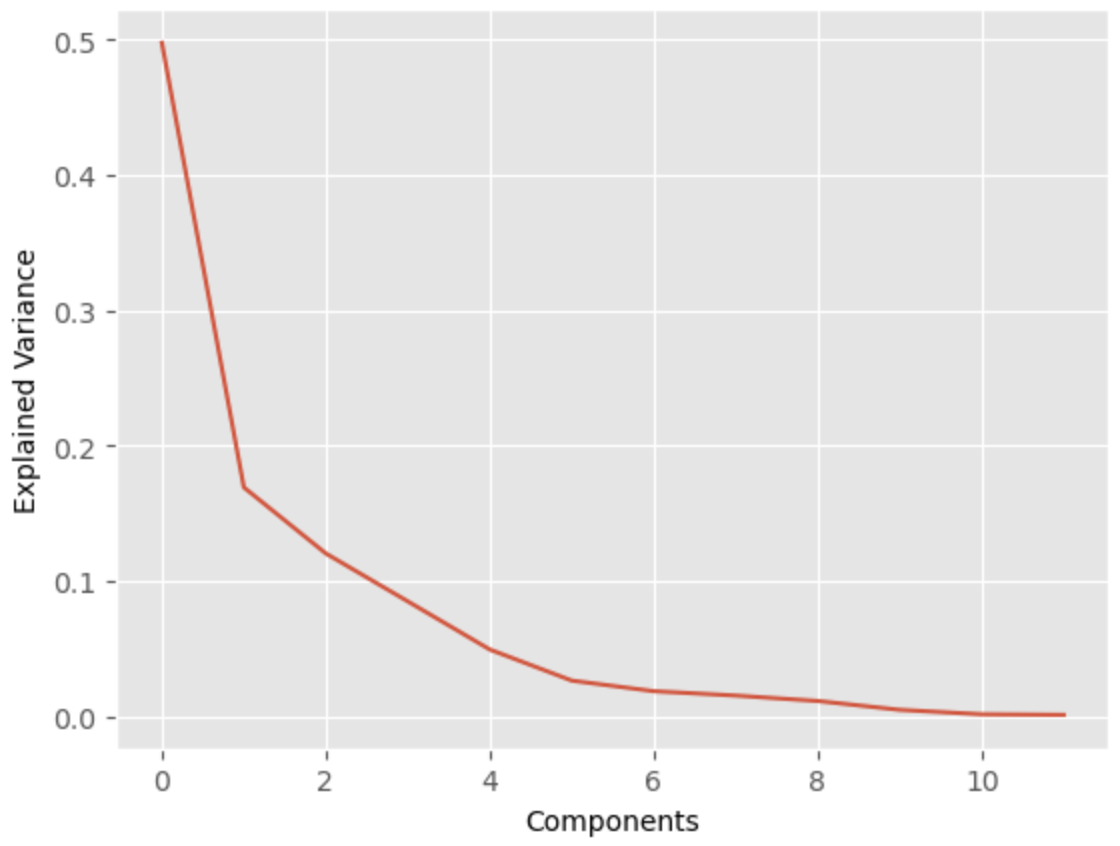
\includegraphics[scale=0.4]{pca.png}
    \caption{Primary component analysis (PCA) on the 12 features in our dataset}
    \label{fig:pca}
\end{figure}

\begin{table*}[]
    \caption{PCA loadings and the corresponding accumulative variance summation for each PC, for features with the correlation $|\rho|>0.5$, which presented in \cref{tab:corr_table}}
    \centering
    \begin{tabular}{l|c|c|c|c|c|c|c|c}
      &   PC0  &  PC1  &  PC2   &  PC3  &  PC4  &  PC5  &  PC6  &  PC7  \\
    \hline
    Bandwidth   & -0.402 & 0.277 & 0.212  & 0.116 & 0.012 & 0.126 & 0.314 & 0.767 \\
    Resolution  & -0.346 & -0.107& -0.667 &	0.201 & -0.453&	-0.411&	0.084 &	0.051 \\
    FPS	        & -0.368 & -0.097& -0.432 & -0.615& 0.495 & 0.201 &	0.071 &-0.016 \\
    Latency     & 0.236	 & 0.636 & -0.240 & 0.189 &	0.504 &	-0.439&	0.002 &-0.005 \\
    Jitter      & 0.273	 & 0.562 & -0.305 & -0.239&	-0.455&	0.502 &	-0.004&-0.014 \\
    PPS         &-0.375  & 0.321 & 0.350  & -0.215& -0.176& -0.215& 0.477 &-0.533 \\
    \makecell[l]{Avg. time\\between packets} & 0.397 & -0.263 & -0.197 & 0.193 & 0.125 & 0.171 & 0.807 & -0.032 \\
    Packets length & -0.394 & 0.102 & -0.113 & 0.626 & 0.205 & 0.504 & -0.102 & -0.351 \\
    \hline
    \hline
    Cumulative variance & 0.648 & 0.827 & 0.907 & 0.944 & 0.967 & 0.990 & 0.998 & 1.\\        

    \end{tabular}

    \label{tab:pca_loadings}
\end{table*}

\begin{figure}
    \centering
    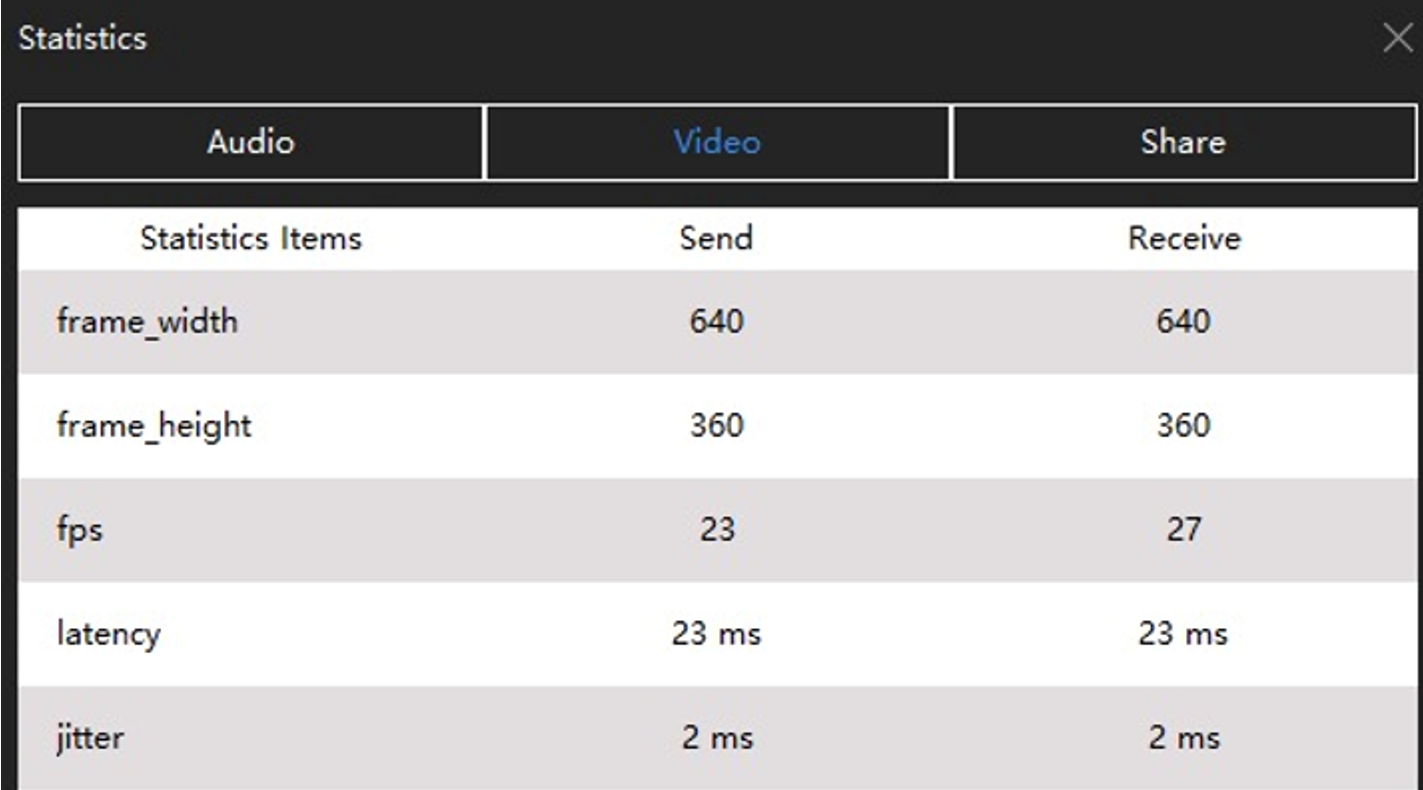
\includegraphics[scale=0.18]{data_examp.png}
    \caption{Zoom quality of experience extracted from an application}
    \label{fig:qoe-from-app}
\end{figure}

\begin{figure}
    \centering
    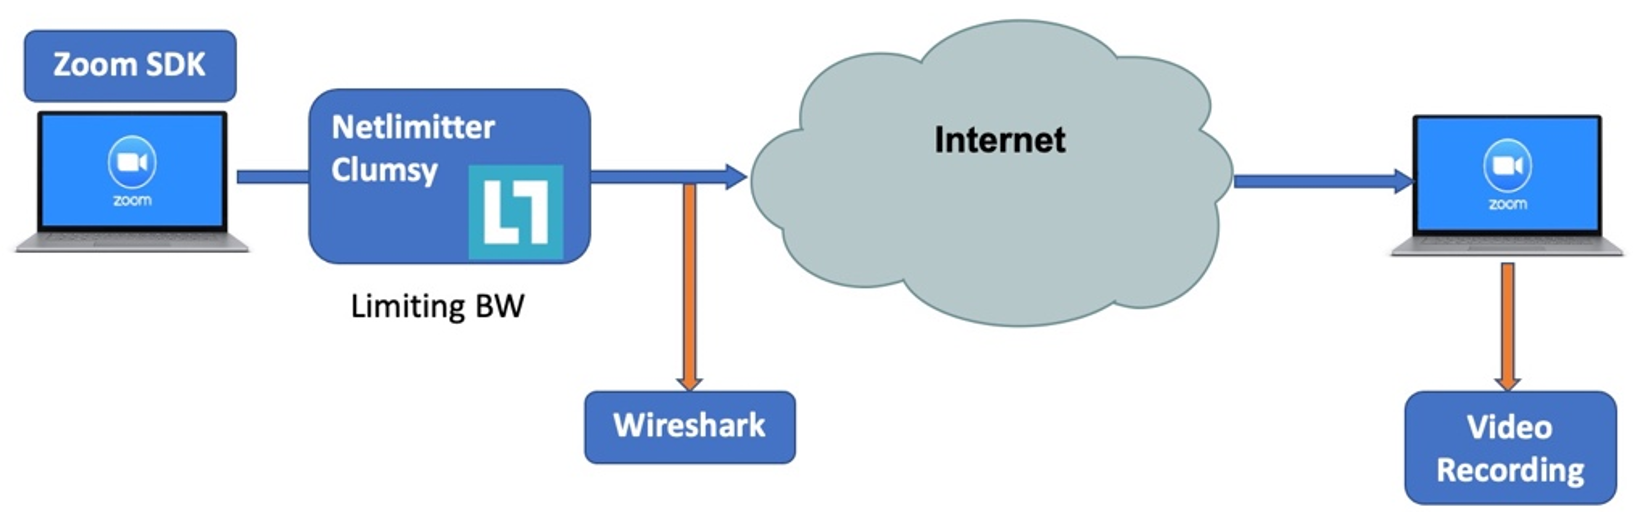
\includegraphics[scale=0.18]{exp_setup.png}
    \caption{Setup used to capture Zoom traffic features and labels}
    \label{fig:exp-setup}
\end{figure}

